\begin{figure}[htb]
\centering
\subfloat[The anticlaw.]{\label{fig:anticlaw}
{\parbox{3.5cm}{
\begin{tikzpicture}[scale = 10]
\tikzstyle{VertexStyle}=[shape = circle,	
								 minimum size = 1pt,
								 inner sep = 1.2pt,
                         draw]
\Vertex[x = 0.131151512265205, y = 0.944127283990383, L = \tiny {$y_1$}]{v0}
\Vertex[x = 0.214424252510071, y = 0.943400021642447, L = \tiny {$y_2$}]{v1}
\Vertex[x = 0.13096971809864, y = 0.849218189716339, L = \tiny {$y_3$}]{v2}
\Vertex[x = 0.214969739317894, y = 0.850490942597389, L = \tiny {$y_4$}]{v3}
\Edge[](v2)(v3)
\Edge[](v2)(v1)
\Edge[](v3)(v1)
\end{tikzpicture}}}}\qquad\qquad
\subfloat[The antidiamond.]{\label{fig:antidiamond}
{\parbox{3.5cm}{
\begin{tikzpicture}[scale = 10]
\tikzstyle{VertexStyle}=[shape = circle,	
								 minimum size = 1pt,
								 inner sep = 1.2pt,
                         draw]
\Vertex[x = 0.131151512265205, y = 0.944127283990383, L = \tiny {$y_1$}]{v0}
\Vertex[x = 0.214424252510071, y = 0.943400021642447, L = \tiny {$y_2$}]{v1}
\Vertex[x = 0.13096971809864, y = 0.849218189716339, L = \tiny {$y_3$}]{v2}
\Vertex[x = 0.214969739317894, y = 0.850490942597389, L = \tiny {$y_4$}]{v3}
\Edge[](v2)(v3)
\end{tikzpicture}}}}
\caption{Labelings of the anticlaw and the antidiamond.}
\end{figure}
